\documentclass[]{article}
\usepackage{lmodern}
\usepackage{amssymb,amsmath}
\usepackage{ifxetex,ifluatex}
\usepackage{fixltx2e} % provides \textsubscript
\ifnum 0\ifxetex 1\fi\ifluatex 1\fi=0 % if pdftex
  \usepackage[T1]{fontenc}
  \usepackage[utf8]{inputenc}
\else % if luatex or xelatex
  \ifxetex
    \usepackage{mathspec}
  \else
    \usepackage{fontspec}
  \fi
  \defaultfontfeatures{Ligatures=TeX,Scale=MatchLowercase}
\fi
% use upquote if available, for straight quotes in verbatim environments
\IfFileExists{upquote.sty}{\usepackage{upquote}}{}
% use microtype if available
\IfFileExists{microtype.sty}{%
\usepackage[]{microtype}
\UseMicrotypeSet[protrusion]{basicmath} % disable protrusion for tt fonts
}{}
\PassOptionsToPackage{hyphens}{url} % url is loaded by hyperref
\usepackage[unicode=true]{hyperref}
\hypersetup{
            pdfborder={0 0 0},
            breaklinks=true}
\urlstyle{same}  % don't use monospace font for urls
\usepackage{graphicx,grffile}
\makeatletter
\def\maxwidth{\ifdim\Gin@nat@width>\linewidth\linewidth\else\Gin@nat@width\fi}
\def\maxheight{\ifdim\Gin@nat@height>\textheight\textheight\else\Gin@nat@height\fi}
\makeatother
% Scale images if necessary, so that they will not overflow the page
% margins by default, and it is still possible to overwrite the defaults
% using explicit options in \includegraphics[width, height, ...]{}
\setkeys{Gin}{width=\maxwidth,height=\maxheight,keepaspectratio}
\IfFileExists{parskip.sty}{%
\usepackage{parskip}
}{% else
\setlength{\parindent}{0pt}
\setlength{\parskip}{6pt plus 2pt minus 1pt}
}
\setlength{\emergencystretch}{3em}  % prevent overfull lines
\providecommand{\tightlist}{%
  \setlength{\itemsep}{0pt}\setlength{\parskip}{0pt}}
\setcounter{secnumdepth}{0}
% Redefines (sub)paragraphs to behave more like sections
\ifx\paragraph\undefined\else
\let\oldparagraph\paragraph
\renewcommand{\paragraph}[1]{\oldparagraph{#1}\mbox{}}
\fi
\ifx\subparagraph\undefined\else
\let\oldsubparagraph\subparagraph
\renewcommand{\subparagraph}[1]{\oldsubparagraph{#1}\mbox{}}
\fi

% set default figure placement to htbp
\makeatletter
\def\fps@figure{htbp}
\makeatother


\date{}

\begin{document}

\begin{quote}
\textbf{Работа 3.2.6}

\textbf{Исследование гальванометра}

\textbf{Цель работы:} изучение работы высокочувствительного зеркального
гальванометра магнитоэлектрической системы в режимах измерения
постоянного тока и электрического заряда.

\textbf{В работе используются:} зеркальный гальванометр с осветителем и
шкалой, источник постоянного напряжения, делитель напряжения, магазин
сопротивлений, эталонный конденсатор, вольтметр, переключатель, ключи,
линейка.
\end{quote}

Баллистическим гальванометром называют электроизмерительный прибор
магнитоэлектрической системы, отличающийся высокой чувствительностью к
току и сравнительно большим периодом колебаний подвижной системы
(рамки).

Главной частью баллистического гальванометра является подвешенная на
вертикальной нити рамка, помещённая в поле постоянного магнита. Вырез
цилиндрической формы в полюсах магнита и ферромагнитный цилиндр на оси
системы делают поле в зазоре радиальным (рис.~1). Скреплённое с рамкой
зеркальце служит для измерения угла поворота рамки. К рамке прикреплён
полый цилиндр, который сильно увеличивает момент инерции и,
следовательно, период колебаний подвижной системы, не очень её утяжеляя.
Магнит и подвижная система заключены в защитный кожух. В баллистических
гальванометрах применяют сильные постоянные магниты и рамки с большим
количеством витков, подвешенные на тонких нитях с малой упругостью.

Баллистический гальванометр позволяет измерять как постоянный ток
(стационарный режим), так и заряд, протекший через рамку за некоторое
время (баллистический режим). В баллистическом режиме гальванометр может
работать, если время протекания заряда много меньше периода собственных
колебаний подвижной рамки. Поэтому период колебаний рамки делают большим
(5~-~15~с). Это время учитывает реакцию экспериментатора, которому надо
успеть сделать отсчёт максимального отклонения рамки.

\textbf{Уравнение движения подвижной системы.} На помещённую в магнитное
поле обтекамую током рамку гальванометра действуют следующие моменты
сил: момент закрученной нити, момент магнитных сил и тормозящий момент,
зависящий от сил сопротивления воздуха и от вихревых токов, вызывающих
электромагнитное торможение. Рассмотрим каждый из этих моментов в
отдельности.

Механический момент \emph{M}\textsubscript{1} упругих сил нити
пропорционален углу поворота рамки:

(1)

где ̶ модуль кручения нити, а ̶ угол поворота рамки от положения
равновесия.

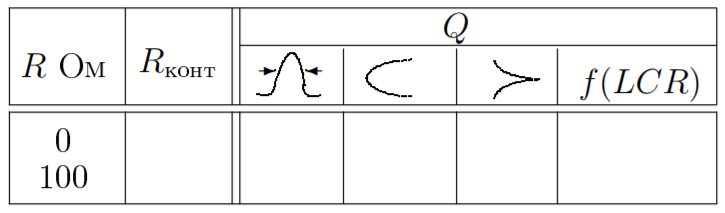
\includegraphics{./media/image4.emf}

Рис. 1. Рамка с током в магнитном поле

Если рамка с числом витков \emph{N}, обтекаемая током \emph{I}, помещена
в магнитное поле с индукцией \emph{B}, то на боковые стороны рамки
(перпендикулярные чертежу на рис. 1) действуют силы, равные \emph{lNBI},
где \emph{l} ̶ длина боковой стороны. Обозначив через расстояние от
боковой стороны до оси вращения, найдём момент пары сил

\begin{quote}
(2)
\end{quote}

где \emph{S} ̶ площадь одного витка рамки.

Тормозящий момент складывается из моментов сил электромагнитного
торможения и сил трения о воздух. В рамке, движущейся в магнитном поле с
угловой скоростью , наводится ЭДС индукции

, (3)

где ̶ магнитный поток, пронизывающий рамку. Пренебрегая самоиндукцией
рамки, можно считать, что эта ЭДС вызывает ток индукции , где -- полное
сопротивление цепи, состоящее из сопротивления рамки и сопротивления
внешнего участка цепи :

(4)

Связанный с ЭДС индукции тормозящий момент

(5)

Обычно этот момент значительно превосходит момент сил трения рамки о
воздух, которым мы и пренебрежём для простоты расчёта.

Уравнение движения рамки , где -- момент инерции подвижной системы, а --
сумма моментов, даваемых формулами (1), (2), (4), представляется в виде:

. (6)

Здесь ток определяется величиной ЭДС внешнего источника, к которому
подключён гальванометр, и полным сопротивлением цепи , а параметры ,
колебательной системы и коэффициент связаны с параметрами гальванометра
формулами:

, , . (7)

Отметим, что заменой переменой на уравнение (6) приводится к однородному
уравнению вида (2.8), описывающему свободные затухающие колебания в
\emph{RCL}-контуре, рассмотренные в теоретической части Раздела II.

\textbf{Режим измерения постоянного тока.} Если через рамку пропускать
постоянный ток (достаточно долго, чтобы затухли колебания подвижной
системы), то в уравнении (6) можно положить , , так что угол поворота
рамки определится формулами

, (8)

где величина называется чувствительностью гальванометра к току, а
обратная её вличина -- постоянной гальванометра.

\textbf{Свободные колебания рамки}. Исследуем свободное движение рамки,
то-есть движение в отсутствие внешних источников тока, когда . В этом
случае уравнение (6) для угла поворота рамки примет вид

, (9)

аналогичный уравнению (2.8), так что мы можем воспользоваться решениями,
полученными в соответствующем разделе сборника, учтя, однако, начальные
условия рассматриваемой здесь задачи. Примем, что эти условия таковы:

, , (10)

то-есть рамке сообщили начальную угловую скорость без заметного
начального смещения. Рассмотрим возможные случаи движения рамки.

1. (колебательный режим).

Решение уравнения (9), удовлетворяющее начальным условиям (10), имеет в
этом случае вид

, . (11)

Движение рамки носит колебательный характер и затухает со временем.
Период колебаний при этом равен

, (12)

а коэффициент затухания определяется формулами (7) и (4). При малом
затухании, когда, , движение рамки близко к синусоидальному:

. (13)

2. (критический режим). Этот режим реализуется при сопротивлении
внешнего участка цепи \emph{R} из формулы (4), равном критическому
сопротивлению

(14)

Решение уравнения (9) при начальных условиях (10) в этом случае имеет
вид

. (15)

Движение не имеет колебательного характера: отклонённая после начального
толчка подвижная система почти экспоненциально возвращается к нулю.

3. (затухание велико ̶ случай переуспокоенного гальванометра). Решение
уравнения (9) при этом имеет вид

, . (16)

Движение остаётся апериодическим, однако подвижная система приближается
к равновесию медленнее, чем в критическом режиме.

\textbf{Режим измерения заряда.} Как уже было отмечено, период свободных
колебаний баллистического гальванометра благодаря искусственному
увеличению момента инерции рамки оказывается очень большим (порядка
десяти секунд). Если пропустить через рамку короткий импульс тока, то
можно считать, что весь ток успевает пройти при неотклонённом положении
рамки. Рамка, однако, при этом получает толчок, в результате которого
возникает движение, описываемое уравнением свободных колебаний (9) при
начальных условиях (10).

Для вычисления угловой скорости , полученной в результате толчка,
проинтегрируем уравнение (6) по времени от 0 до ̶ момента окончания
токового импульса. В результате приходим к соотношению

, (17)

где ̶ полный электрический заряд, прошедший через рамку гальванометра за
время импульса. При малом начальном отклонении рамки и малой
длительности импульса можно пренебречь вторым и третьим слагаемыми в
(16), связанными соответственно с током индукции и упругостью нити.
Уравнение (16) в этом случае принимает вид:

. (18)

Таким образом, при пропускании короткого импульса тока через
баллистический гальванометр начальная угловая скорость движения рамки
пропорциональна полному электрическому заряду, прошедшему через рамку за
всё время импульса. Подставляя выражения (11), (14) или (15), легко
увидеть, что наибольший угол, на который отклоняется рамка, также
пропорционален .

Величина называется баллистической постоянной гальванометра.
Баллистическая постоянная наряду с динамической является важнейшей
характеристикой гальванометра, но в отличие от динамической она
существенно зависит от режима работы гальванометра (от сопротивления
цепи). Величина называется чувствительностью гальванометра к
заряду\textbf{.}

Выбирая оптимальный режим работы, приходится одновременно исходить из
двух противоречивых требований: желания получить максимальную
чувствительность гальванометра к заряду и стремления по возможности
сократить время, затрачиваемое на измерения.

Расчёт показывает, что максимальный отброс достигается при полном
отсутствии затухания (тормозящий индукционный ток отсутствует при обрыве
в цепи):

. (19)

В этом случае, однако, возникшие в результате отброса колебания рамки не
будут успокаиваться, и прибор не скоро сможет быть использован для
повторных измерений. Поэтому обычно заботятся о том, чтобы затухание
гальванометра не было слишком малым. Кроме того, отметим, что затухание
приводит к тому, что зайчик начинает вести себя более спокойно и слабее
реагирует на посторонние электрические и механические импульсы.

Обычно удобнее всего работать в режиме, близком к критическому. При этом
обеспечивается быстрое затухание колебаний, и чувствительность прибора
достаточно велика.

Как следует из уравнения (14), в случае критического затухания

. (20)

Таким образом, в критическом режиме максимальное отклонение зайчика в
раз меньше, чем в режиме свободных колебаний. Отсюда, в частности,
следуют соотношения

(21)

между баллистическими постоянными и чувствительностями гальванометра,
работающего в режиме свободных колебаний (св) и в критическом (кр)
режиме.

\textbf{A. Определение динамической постоянной гальванометра}

\textbf{Экспериментальная установка.} Схема для исследования
гальванометра в стационарном режиме представлена на рис. 2. Постоянное
напряжение В снимается с блока питания и измеряется вольтметром V. Ключ
позволяет менять направление тока через гальванометр Г, делитель
напряжения ̶ менять величину тока в широких пределах. Ключ служит для
включения гальванометра, кнопка ̶ для его успокоения. Магазин
сопротивлений \emph{R} позволяет менять режим работы гальванометра от
колебательного до апериодического.

\includegraphics{./media/image71.emf}

Рис. 2. Схема установки для работы гальванометра в стационарном режиме

При сила тока, протекающего через гальванометр, может быть вычислена по
очевидной формуле:

, (22)

где ̶ показания вольтметра, ̶ положение делителя, ̶ сопротивление магазина,
̶ внутреннее сопротивление гальванометра.

Угол отклонения рамки от положения равновесия измеряется с помощью
осветителя, зеркальца, укреплённого на рамке, и шкалы, на которую
отбрасывается луч света от зеркальца. Координата светового пятна на
шкале связана с углом отклонения рамки формулой

, (23)

где ̶ расстояние от шкалы до зеркальца. При малых углах можно считать,
что . Динамическую постоянную

, (24)

как правило, выражают в единицах (ток измеряется в амперах, ̶ в мм, ̶ в
метрах).

\textbf{Б. Определение критического сопротивления гальванометра}

Критическим сопротивлением баллистического гальванометра называется
сопротивление его электрической цепи , при котором после начального
толчка подвижная система почти экспоненциально возвращается к нулю,
подчиняясь уравнению (14). Как отмечалось в теоретическом введении к
Разделу II, на практике критический режим, требующий строгого выполнения
условия , не может быть точно реализован и имеет значение как
пограничный между режимом затухающих колебаний () и режимом
апериодического затухания .

Измерение критического сопротивления гальванометра можно выполнить с
помощью той же схемы (рис.~2).

При больших \emph{R} свободное движение рамки имеет колебательный
характер. С уменьшением \emph{R} затухание увеличивается (см. (4), (7)),
и колебательный режим переходит в апериодический.

В качестве характеристики процесса затухания колебаний рамки
гальванометра воспользуемся представленым формулой (2.25)
логарифмическим декрементом затухания

, (25)

где и -- два последовательные отклонения колеблющейся величины в одну
сторону. Измеряя зависимость логарифмического декремента затухания от
сопротивления внешней цепи , можно найти критическое сопротивление по
формуле, которая следует из выражений (14) и (25):

. (26)

Напомним, что сопротивление связано с параметрами баллистического
гальванометра формулой (14).

\textbf{В. Определение баллистической постоянной и критического
сопротивления гальванометра, работающего в баллистическом режиме}

Для изучения работы гальванометра в режиме измерения заряда, а значит, в
баллистическом режиме, используется схема, представленная на pис.~3.

Система ключей устроена так, что нормально ключ
\emph{K}\textsubscript{2} замкнут, а ключи \emph{K}\textsubscript{3} и
\emph{K}\textsubscript{4} разомкнуты. При нажатии на кнопку
\emph{K}\textsubscript{0} сначала размыкается ключ
\emph{K}\textsubscript{2}, затем замыкается \emph{K}\textsubscript{3} и
через некоторое время ̶ \emph{K}\textsubscript{4}. При нормальном
положении кнопки \emph{K}\textsubscript{0} конденсатор \emph{C}
заряжается до напряжения и получает заряд :

, . (27)

При нажатии на ключ \emph{K}\textsubscript{0} конденсатор отключается от
источника постоянного напряжения (размыкается ключ
\emph{K}\textsubscript{2}) и подключается к гальванометру (замыкается
ключ \emph{K}\textsubscript{3}).

\includegraphics{./media/image104.emf}

Рис. 3. Схема установки для определения баллистической постоянной

Ёмкость конденсатора выбрана так, что к моменту замыкания ключа
\emph{K}\textsubscript{4} весь заряд успевает пройти через гальванометр,
и рамка получает начальную скорость (см.~(18)). При этом можно считать,
что отклонение рамки, происходящее за время, протекающее между
замыканием ключей \emph{K}\textsubscript{3} и \emph{K}\textsubscript{4},
равно нулю. При замыкании ключа \emph{K}\textsubscript{4} гальванометр
шунтируется внешним сопротивлением \emph{R}, и в зависимости от величины
этого сопротивления движение рамки описывается одним из уравнений: (11),
(13), (15) или (16).

Первый отброс зайчика после нажатия на кнопку \emph{K}\textsubscript{0}
зависит от сопротивления внешней цепи, подключённой к гальванометру. Для
определения \emph{R}\textsubscript{кр} используется то обстоятельство,
что в критическом режиме максимальное отклонение зайчика в раз меньше,
чем у гальванометра без затухания (см. (17) и (18)).

Следует помнить, что наблюдать колебания рамки при полном отсутствии
затухания, конечно, невозможно, так как даже при разомкнутой внешней
цепи () остаётся трение в подвеске и трение рамки о воздух. Величину
максимального отклонения рамки гальванометра без затухания можно,
однако, рассчитать, если при разомкнутой цепи измерены максимальное
отклонение рамки и логарифмический декремент затухания . Из уравнений
(11) и (25) при вытекают равенства

, (28)

так что максимальное отклонение рамки гальванометра без затухания

(29)

Баллистическая постоянная гальванометра определяется при критическом
сопротивлении ():

, (30)

где ̶ величина первого отброса в критическом режиме, выраженная в
делениях шкалы (мм), ̶ расстояние от зеркальца до шкалы, выраженное в
метрах, произведение ̶ заряд, выраженный в кулонах.

\textbf{ЗАДАНИЕ}

В работе предлагается определить динамическую постоянную , критическое
сопротивление и оценить линейность шкалы гальванометра, работающего в
стационарном (токовом) режиме; определить баллистическую постоянную и
критическое сопротивление гальванометра, работающего в баллистическом
режиме (режиме измерения заряда).

I. Подготовка приборов к работе

1.~Настройте осветитель гальванометра: для этого перемещая штатив со
шкалой вдоль луча, добейтесь появления на шкале чёткой вертикальной
риски. Перемещая штатив (или шкалу) перпендикулярно лучу, совместите
риску с нулевым делением шкалы. Настроив, временно отключите осветитель
от сети.

2.~Установите делитель на небольшое выходное напряжение ( или ), а
сопротивление магазина установите близким к максимальному ( кОм).

3.~Соберите электрическую цепь согласно pис.~2 (кнопка
\emph{K}\textsubscript{1} вмонтирована в блок питания!).

4.~При разомкнутых ключах \emph{K}\textsubscript{2} и
\emph{K}\textsubscript{3} включите в сеть блок питания и, убедившись,
что шкала вольтметра \emph{V} выбрана правильно, замкните ключ
\emph{K}\textsubscript{3}.

5.~Включите осветитель гальванометра.

6.~Замкните ключ \emph{K}\textsubscript{2} и, не меняя положения
делителя, подберите сопротивление магазина, при котором зайчик
отклоняется почти на всю шкалу.

II. Определение динамической постоянной

7.~Снимите зависимость отклонения зайчика \emph{x} от сопротивления
магазина \emph{R}, увеличивая сопротивление магазина, но не меняя
делителя. Запишите показания вольтметра \emph{U}\textsubscript{0},
положение делителя \emph{R}\textsubscript{1}\emph{/R}\textsubscript{2},
величину \emph{R}\textsubscript{2} и внутреннее сопротивление
гальванометра \emph{R}\textsubscript{0}, указанное на установке.

III. Определение критического сопротивления

8.~В схеме, собранной по pис.~2, вновь установите такое значение
\emph{R}, при котором зайчик отклоняется почти на всю шкалу.

9.~Разомкните ключ \emph{K}\textsubscript{2} и наблюдайте свободные
колебания рамки. Для быстрого торможения рамки замыкайте ключ
\emph{K}\textsubscript{3} в момент прохождения зайчика через ноль.
Измерьте два последовательных отклонения зайчика в одну сторону для
расчёта логарифмического декремента затухания разомкнутого гальванометра
(см. (25)).

10.~Измерьте период \emph{T}\textsubscript{0} свободных колебаний рамки
(приближённо).

11.~Снова замкните ключ \emph{K}\textsubscript{2} и убедитесь, что
зайчик находится на краю шкалы. Теперь разомкните ключ
\emph{K}\textsubscript{3}. Колебания рамки затухнут быстрее, так как
тормозящий движение ток увеличился с уменьшением сопротивления цепи.

12.~Подберите \emph{наибольшее} сопротивление магазина \emph{R}, при
котором при размыкании ключа \emph{K}\textsubscript{3} зайчик не
переходит за нулевое значение (при этом для большей точности каждый раз
следует подбирать положение делителя так, чтобы в стационарном положении
зайчик отклонялся почти на всю шкалу). Это наибольшее сопротивление
близко к критическому сопротивлению .

13.~Установите сопротивление магазина (близкое целое) и подберите
делитель так, чтобы в стационарном режиме зайчик отклонялся почти на всю
шкалу. Для расчёта декремента затухания измерьте два последовательных
отклонения зайчика в одну сторону после размыкания ключа
\emph{K}\textsubscript{3}.

14.~Повторите измерения п.13 для 8 ̶ 10 других значений \emph{R},
постепенно увеличивая сопротивление магазина до (в интервале (3 ̶ 6)
точки должны лежать почаще).

IV. Баллистический режим

15.~Соберите схему по pис.~3. Установите на магазине сопротивление
\emph{R}=50 кОм. Включите в сеть блок питания и замкните ключ
\emph{K}\textsubscript{5}.

16.~Для измерения первого отброса зайчика в режиме свободных колебаний
() разомкните цепь \emph{R}, отсоединив одну из клемм от магазина.

Подберите делитель так, чтобы при замыкании ключа
\emph{K}\textsubscript{0} первый отброс соответствовал отклонению
зайчика почти на всю шкалу (ключ \emph{K}\textsubscript{0} держите
замкнутым, когда считываете результат!).

17.~Вновь подключите магазин \emph{R}. Не меняя положения делителя,
снимите зависимость первого отброса от величины \emph{R}. В критическом
режиме первый отброс в \emph{e} раз меньше, чем в режиме свободных
колебаний. Поэтому уменьшайте \emph{R} до тех пор, пока первый отброс
уменьшится до 1/3 ̶ 1/4 от максимальной величины.

18.~Запишите положение делителя
\emph{R}\textsubscript{1}\emph{/R}\textsubscript{2} и значение ёмкости
\emph{C}. Измерьте расстояние \emph{a} от шкалы до зеркальца
гальванометра.

19.~Разберите схему.

V. Обработка результатов

20.~По данным п.~7 рассчитайте токи \emph{I} по формуле (22) и постройте
график \emph{I=f(x)}. Оцените линейность шкалы гальванометра. По наклону
прямой рассчитайте динамическую постоянную {[}A/(мм/м){]} по формуле
(24), а также чувствительность гальванометра к току {[}(мм/м)/A{]}.

21.~По данным пп.~8,~9 рассчитайте логарифмический декремент затухания
разомкнутого гальванометра по формуле (25).

22.~По данным пп.~12~ ̶ ~14 составьте таблицу, в первой строке которой
внесите 7~ ̶ ~10 выбранных значений \emph{R}, во второй ̶ соответствующие
этим значениям \emph{R} измеренные величины , в третьей строке ̶
рассчитанные по формуле (26) значения . Результат косвенного измерения
величины критического сопротивления гальванометра представьте в виде ,
где ̶ среднее значение , ̶ случайная погрешностсь, а ̶ коэффициент
Стьюдента для доверительного уровня и числа измерений \emph{n}.

23.~Постройте график . Определите по графику критическое сопротивление
гальванометра (с учётом (29)).

24.~Сравните значения , определённые подбором (п.~12), по результатам
п.~22 для стационарного режима и по графику для баллистического режима.

25.~Рассчитайте баллистическую постоянную в критическом режиме
{[}Кл/(мм/м){]} по формуле (30).

26.~Сравните период свободных колебаний гальванометра
\emph{T}\textsubscript{0} (п.10) и время релаксации .

\textbf{Контрольные вопросы}

1.~Дайте определение динамической постоянной гальванометра. От чего она
зависит и в каких единицах указывается в паспорте гальванометра?

2.~Какие режимы движения рамки возможны при работе гальванометра в
стационарном режиме? В каком из этих режимов удобно проводить измерения
постоянного тока?

3.~Как изменяется коэффициент затухания подвижной системы гальванометра
при увеличении омического сопротивления его цепи?

4.~Почему рамка гальванометра быстро успокаивается при замыкании ключа
\emph{K}\textsubscript{1} (см. pис. 2)?

5.~Зачем в полюсах магнита гальванометра делают вырез цилиндрической
формы? (pис.~1)

6.~В чём сущность баллистического режима работы гальванометра? Дайте
определение баллистической постоянной гальванометра.

7.~При каких условиях первый отброс гальванометра, работающего в
баллистическом режиме, максимален?

8.~При значениях \emph{R}\textgreater{}10\emph{R}\textsubscript{кр}
возможно заметное отклонение значений критического сопротивления от ,
полученного в п.~22. Что следовало бы учесть для объяснения этого
отклонения?

СПИСОК ЛИТЕРАТУРЫ

1.~Сивухин Д.В. Общий курс физики. Т.~III. Электричество. М.: ФИЗМАТЛИТ,
2006, §~125.

2.~Калашников С.Г. Электричество. М.: ФИЗМАТЛИТ, 2003, §~56.

\end{document}
